\section{Hilbert空间中的有限观测拟合}
\label{sec:opt-fit-hilbert}

前两节先固定了有限个基函数，再求系数。基函数选多少、选哪些，本身就是一个限制：真正好的函数可能不在它们张成的空间里。现在反过来，让候选取遍一个无限维Hilbert空间$H$，只保留读数是有限个这一事实。本节说明，在这一设定下，有限个读数会自动把搜索压缩到一个有限维子空间；所得的有限维问题可以用Gram矩阵写出，并在正则化与精确插值两种任务下讨论解的存在与唯一。

\subsection{正交分解与表示定理}
\label{sec:opt-fit-representer}

\paragraph{读数只看见有限个方向}
设$H$是实Hilbert空间，$L_1,\dots,L_n$是$H$上的有界线性泛函。由Riesz表示定理，每个$L_i$对应唯一的$h_i\in H$，使$L_if=\langle f,h_i\rangle_H$对一切$f\in H$成立；有界线性泛函与Riesz表示的一般理论可参考\BookChapterRef{chap:linear-functionals-operators}{卷二“线性泛函与线性算子”章}。在再生核Hilbert空间中读点值$f(x_i)$时，表示元就是核截面$h_i=K(\cdot,x_i)$；对有界连续核与有限测度$\nu$读积分$\int f\varphi_i\,\mathrm d\nu$（$\varphi_i\in L^2(\nu)$）时，表示元是$h_i=\int K(\cdot,x)\varphi_i(x)\,\mathrm d\nu(x)$，它一般不是任何一个核截面。

令$M=\operatorname{span}\{h_1,\dots,h_n\}$。它是有限维子空间，因而是闭的，到它的正交投影$P_M$存在；Hilbert空间中闭子空间的投影定理可参考\BookChapterRef{chap:function-spaces}{卷二“函数空间”章}。把任一$f\in H$分解为
\[
  f=P_Mf+r,\qquad r\perp M .
\]
余项$r$与每个$h_i$正交，所以$L_ir=\langle r,h_i\rangle=0$，即$Lf=L(P_Mf)$：去掉余项，读数一个也不变。同时由勾股定理$\|f\|_H^2=\|P_Mf\|_H^2+\|r\|_H^2\ge\|P_Mf\|_H^2$，投影不增大范数，且仅当$r=0$时范数不变。图~\ref{fig:opt-fit-representer-geometry}把这件事画成平面图：与$f$读数相同的候选组成一条与$M$垂直的直线，它与$M$的交点$P_Mf$是这条直线上离原点最近的点。

\begin{figure}[!htbp]
  \centering
  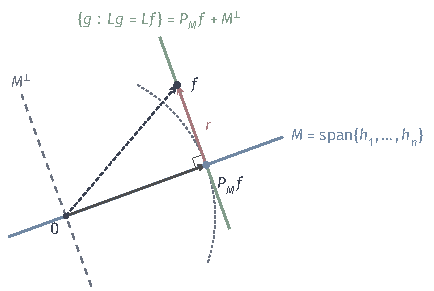
\includegraphics[width=73.5mm]{figures/03-optimization-evolution-and-signals/01-optimization/tikz/c8-representer-geometry/figure.pdf}
  \caption{表示定理的几何。蓝线为观测表示元张成的子空间$M$，灰色虚线为其正交补$M^\perp$；与$f$读数相同的全部候选组成仿射集$P_Mf+M^\perp$（绿线）。余项$r=f-P_Mf$垂直于$M$，不改变任何读数；以原点为心、过$P_Mf$的圆弧（灰色点线）与绿线相切，说明$P_Mf$是该仿射集中范数最小的元素。}
  \label{fig:opt-fit-representer-geometry}
\end{figure}

\paragraph{表示定理}
考虑一般的正则化拟合目标
\begin{equation}
  \min_{f\in H}\ J(f)=\Phi(Lf)+\Omega\bigl(\|f\|_H\bigr),
  \label{eq:opt-fit-representer-problem}
\end{equation}
其中$\Phi:\mathbb R^n\to\mathbb R\cup\{+\infty\}$是任意的数据代价（数据$\bm y$已含在$\Phi$中），$\Omega:[0,\infty)\to\mathbb R$单调不减。上面的两条观察直接给出$J(P_Mf)\le J(f)$：数据项不变，正则项不增。

\begin{theorem}[表示定理]
\label{thm:opt-fit-representer}
在上述设定下：
\begin{enumerate}
  \item $\inf_{f\in H}J(f)=\inf_{f\in M}J(f)$；
  \item 若$J$在某个$f^\star\in H$处达到最小值，则$P_Mf^\star\in M$也是最小点；
  \item 若$\Omega$严格递增，且最小值有限，则每个最小点都属于$M$，即都形如$\sum_{j=1}^na_jh_j$。
\end{enumerate}
\end{theorem}

\begin{proof}
(1) $M\subseteq H$给出$\inf_HJ\le\inf_MJ$。反过来，对任意$f\in H$，$P_Mf\in M$且$J(P_Mf)\le J(f)$，所以$\inf_MJ\le J(f)$，对$f$取下确界得$\inf_MJ\le\inf_HJ$。

(2) $J(P_Mf^\star)\le J(f^\star)=\min_HJ$，而$P_Mf^\star\in H$，所以等号成立。

(3) 设$f^\star$是最小点而$r=f^\star-P_Mf^\star\ne0$。则$\|P_Mf^\star\|_H<\|f^\star\|_H$，$\Omega$严格递增给出$\Omega(\|P_Mf^\star\|)<\Omega(\|f^\star\|)$，数据项相同，于是$J(P_Mf^\star)<J(f^\star)$，与$f^\star$是最小点矛盾（这里用到$J(f^\star)$有限）。
\end{proof}

这一结论称为\term{表示定理}（representer theorem）\scite{scholkopf2001representer}。它把一个无限维的搜索化成了$n$个系数$a_1,\dots,a_n$的搜索，代价是要知道表示元$h_i$及它们的内积。

\paragraph{定理没有说的事}
定理的三条结论都是有条件的。第1条只比较下确界，没有说最小值能达到；第2条在“若达到”的前提下才给出$M$中的最小点；第3条在$\Omega$只是单调不减（例如在某段上为常数）时可能不成立，此时$M$外也可以有最小点。最小点是否存在、是否唯一，要像下一小节那样另外证明。

候选集合另加约束时，还要检查投影是否保持可行。若约束只涉及同一组读数，例如$L_1f\ge0$，那么$P_Mf$与$f$读数相同，可行性不变。若约束涉及$M$以外的信息，结论可能失效。在$[0,1]$上以最小值核$K(s,t)=\min(s,t)$生成的空间$H_{\min}$中（其范数为$\|f\|_H^2=\int_0^1(f')^2\,\mathrm dx$，要求$f(0)=0$），只读一个点值$f(\tfrac12)=0$，于是$M=\operatorname{span}\{\min(\cdot,\tfrac12)\}$；若再要求$f(\tfrac14)\ge1$，任何可行的$f$投影后都变成$P_Mf=c\min(\cdot,\tfrac12)$，由$c/2=f(\tfrac12)=0$得$P_Mf=0$，不再满足$f(\tfrac14)\ge1$。此时最优解不必落在$M$中，约束$f(\tfrac14)\ge1$本身也是一个读数，应把它的表示元加进$M$。

\subsection{Gram矩阵与正则化平方拟合}
\label{sec:opt-fit-gram}

\paragraph{有限维问题的系数形式}
在$M$中写$f=\sum_{j=1}^na_jh_j$，$\bm a\in\mathbb R^n$。记\term{Gram矩阵}（Gram matrix）$\bm G_{i,j}=\langle h_i,h_j\rangle_H=L_ih_j$，它对称半正定。读数与范数都由它算出：
\begin{equation}
  L_if=\sum_ja_j\langle h_j,h_i\rangle=(\bm G\bm a)_i,\qquad
  \|f\|_H^2=\sum_{i,j}a_ia_j\langle h_i,h_j\rangle=\bm a^\top\bm G\bm a .
  \label{eq:opt-fit-gram-calculus}
\end{equation}
读点值时$\bm G_{i,j}=K(x_i,x_j)$，就是\term{核矩阵}（kernel matrix）；读积分等一般观测时，$\bm G$仍是表示元的Gram矩阵，但不再是核在观测点上的取值。

现在取平方数据代价与平方范数正则，$\lambda>0$：
\begin{equation}
  J(f)=\frac1n\|Lf-\bm y\|_2^2+\lambda\|f\|_H^2 .
  \label{eq:opt-fit-kernel-ridge}
\end{equation}
点值观测下，这就是\term{核岭回归}（kernel ridge regression）。由式~\eqref{eq:opt-fit-gram-calculus}，它在$M$上的系数形式是
\[
  J(\bm a)=\frac1n\|\bm G\bm a-\bm y\|_2^2+\lambda\,\bm a^\top\bm G\bm a ,\qquad
  \nabla J(\bm a)=\frac2n\bm G\bigl[(\bm G+n\lambda\bm I)\bm a-\bm y\bigr].
\]
梯度为零的条件是
\begin{equation}
  \bm G\bigl[(\bm G+n\lambda\bm I)\bm a-\bm y\bigr]=\bm 0 .
  \label{eq:opt-fit-kernel-stationary}
\end{equation}
$\bm G+n\lambda\bm I$对称正定，所以$\bm a_\lambda=(\bm G+n\lambda\bm I)^{-1}\bm y$满足它。称这个解为规范代表，它满足的方程$(\bm G+n\lambda\bm I)\bm a=\bm y$比式~\eqref{eq:opt-fit-kernel-stationary}更强。

\begin{theorem}[正则化平方拟合的解]
\label{thm:opt-fit-kernel-ridge}
设$L_i$有界，$\lambda>0$。则目标~\eqref{eq:opt-fit-kernel-ridge}在$H$上有唯一的最小点
\[
  f_\lambda=\sum_{j=1}^n(a_\lambda)_jh_j,\qquad \bm a_\lambda=(\bm G+n\lambda\bm I)^{-1}\bm y .
\]
满足式~\eqref{eq:opt-fit-kernel-stationary}的任一系数向量都给出同一个函数$f_\lambda$。
\end{theorem}

\begin{proof}
$J(\bm a)$是$\bm a$的凸二次函数（Hessian为$\tfrac2n\bm G^2+2\lambda\bm G\succeq\bm0$），所以满足式~\eqref{eq:opt-fit-kernel-stationary}的点都是它在$\mathbb R^n$上的最小点；$\bm a_\lambda$是其中之一，于是$f_\lambda$在$M$上达到最小。由表示定理第1条，$f_\lambda$也是$H$上的最小点。$\Omega(t)=\lambda t^2$在$[0,\infty)$上严格递增，由第3条，$H$上的每个最小点都在$M$中，形如$\sum_ja_jh_j$，其系数是$J(\bm a)$的最小点，因而满足式~\eqref{eq:opt-fit-kernel-stationary}。

剩下证明满足式~\eqref{eq:opt-fit-kernel-stationary}的两个系数$\bm a,\bm a'$给出同一函数。令$\bm d=\bm a-\bm a'$，相减得$\bm G(\bm G+n\lambda\bm I)\bm d=\bm 0$。左乘$\bm d^\top$，得$\|\bm G\bm d\|_2^2+n\lambda\,\bm d^\top\bm G\bm d=0$；两项都非负，故$\bm d^\top\bm G\bm d=0$。由式~\eqref{eq:opt-fit-gram-calculus}，这正是$\bigl\|\sum_jd_jh_j\bigr\|_H^2=0$，两组系数代表同一个函数。
\end{proof}

\paragraph{函数唯一不等于系数唯一}
定理中唯一的是函数，不是系数。$\bm G$奇异时，系数可以沿$\ker\bm G$任意移动而函数不变：若$\bm G\bm d=\bm 0$，则$\|\sum_jd_jh_j\|^2=\bm d^\top\bm G\bm d=0$。例如在$[-1,1]$上取仿射核$K(s,t)=1+st$，读三个点值$x=-1,0,1$，核截面$1-x$、$1$、$1+x$线性相关，$\bm G=\bigl[\begin{smallmatrix}2&1&0\\1&1&1\\0&1&2\end{smallmatrix}\bigr]$，$\ker\bm G=\operatorname{span}\{(1,-2,1)^\top\}$，对应的函数组合$(1-x)-2+(1+x)$恒为零。规范代表$\bm a_\lambda$是满足更强方程的那一个；其他满足式~\eqref{eq:opt-fit-kernel-stationary}的系数都与它相差$\ker\bm G$中的向量。数值上应以Cholesky分解求解$(\bm G+n\lambda\bm I)\bm a=\bm y$，而不显式求逆；后者多花计算，也放大舍入误差。

\begin{example}[最小值核上的两点拟合]
\label{ex:opt-fit-min-kernel}
在$H_{\min}$中读$f(\tfrac12)=1$、$f(1)=1$，$n=2$。核截面$K_{1/2}=\min(\cdot,\tfrac12)$与$K_1=\min(\cdot,1)$都是从原点出发的折线，Gram矩阵$\bm G=\bigl[\begin{smallmatrix}1/2&1/2\\1/2&1\end{smallmatrix}\bigr]$。取$\lambda=\tfrac14$，$n\lambda=\tfrac12$，
\[
  \bm G+\tfrac12\bm I=\begin{bmatrix}1&1/2\\1/2&3/2\end{bmatrix},\qquad
  \bm a_\lambda=\frac45\begin{bmatrix}3/2&-1/2\\-1/2&1\end{bmatrix}\begin{bmatrix}1\\1\end{bmatrix}=\begin{bmatrix}4/5\\2/5\end{bmatrix}.
\]
拟合函数$f_\lambda=\tfrac45\min(\cdot,\tfrac12)+\tfrac25\min(\cdot,1)$在$[0,\tfrac12]$上斜率为$\tfrac65$，在$[\tfrac12,1]$上斜率为$\tfrac25$。读数$\bm G\bm a_\lambda=(\tfrac35,\tfrac45)^\top$，都比数据$1$小；范数平方$\bm a_\lambda^\top\bm G\bm a_\lambda=\tfrac45$。图~\ref{fig:opt-fit-min-kernel}(a)画出了两条核截面（灰色点线）及其组合（蓝线）：正则化让函数以较小的范数为代价，在读数上作了让步。
\end{example}

\subsection{最小范数插值}
\label{sec:opt-fit-min-norm-interpolation}

把正则化拟合换成必须精确满足读数的任务：
\[
  \min_{f\in H}\ \|f\|_H\qquad\text{s.t.}\quad Lf=\bm y .
\]
它的解称为\term{最小范数插值}（minimum-norm interpolation）。首先要判断约束是否可满足。由$Lf=L(P_Mf)$及式~\eqref{eq:opt-fit-gram-calculus}，$L$的像集等于$\{\bm G\bm a:\bm a\in\mathbb R^n\}=\operatorname{range}\bm G$，所以插值有解当且仅当$\bm y\in\operatorname{range}\bm G$。读数不相容时问题没有可行点；此时求$\min_f\|Lf-\bm y\|$得到的是最小二乘拟合，它的残差不为零，不能当作插值。

\begin{theorem}[最小范数插值]
\label{thm:opt-fit-min-norm-interpolation}
设$\bm y\in\operatorname{range}\bm G$，令$\bm a^\dagger=\bm G^\dagger\bm y$、$f^\dagger=\sum_ja^\dagger_jh_j$。则$f^\dagger$插值数据，并且是唯一的最小范数插值函数，$\|f^\dagger\|_H^2=\bm y^\top\bm G^\dagger\bm y$。任一满足$\bm G\bm a=\bm y$的系数都给出同一函数$f^\dagger$。
\end{theorem}

\begin{proof}
$\bm G\bm G^\dagger$是到$\operatorname{range}\bm G$的正交投影，$\bm y$在其中，所以$Lf^\dagger=\bm G\bm a^\dagger=\bm y$。若$g\in H$也满足$Lg=\bm y$，则$\langle g-f^\dagger,h_i\rangle=L_i(g-f^\dagger)=0$对每个$i$成立，即$g-f^\dagger\perp M$；而$f^\dagger\in M$，由勾股定理$\|g\|_H^2=\|f^\dagger\|_H^2+\|g-f^\dagger\|_H^2\ge\|f^\dagger\|_H^2$，等号当且仅当$g=f^\dagger$。范数由$\bm a^{\dagger\top}\bm G\bm a^\dagger=\bm y^\top\bm G^\dagger\bm G\bm G^\dagger\bm y=\bm y^\top\bm G^\dagger\bm y$得到。最后，若$\bm G\bm a=\bm y=\bm G\bm a^\dagger$，则$\bm G(\bm a-\bm a^\dagger)=\bm 0$，上一小节已说明这样的两组系数给出同一函数。
\end{proof}

伪逆在系数层面选出欧氏长度最小的一组系数，但定理中的“最小范数”指函数的$H$范数，与选哪组系数无关。对点值观测，这与卷二“再生核Hilbert空间”章中观测投影的最小范数性质一致。

继续例~\ref{ex:opt-fit-min-kernel}。$\bm G$可逆，$\bm a^\dagger=\bm G^{-1}\bm y=4\bigl[\begin{smallmatrix}1&-1/2\\-1/2&1/2\end{smallmatrix}\bigr](1,1)^\top=(2,0)^\top$，于是$f^\dagger=2\min(\cdot,\tfrac12)$：从原点以斜率$2$升到$(\tfrac12,1)$，之后保持水平，$\|f^\dagger\|_H^2=\int_0^{1/2}4\,\mathrm dx=2$。另取$r(x)=\tfrac14\sin2\pi x$，它满足$r(0)=r(\tfrac12)=r(1)=0$，因而$r\perp M$，$f^\dagger+r$也插值数据，范数平方却是$2+\int_0^1(\tfrac\pi2\cos2\pi x)^2\,\mathrm dx=2+\tfrac{\pi^2}8\approx3.23$。图~\ref{fig:opt-fit-min-kernel}(b)画出这两个读数相同的插值函数：多出来的波动不被读数察觉，只增加范数。比较(a)中的红色虚线，正则化解$f_\lambda$在$\lambda\downarrow0$时趋于$f^\dagger$，第~\ref{sec:opt-fit-lambda}小节会证明这一点。

再看仿射核的例子，$\operatorname{range}\bm G=\{(1,-2,1)^\top\}^\perp$。读数$\bm y=(0,0,1)^\top$与$(1,-2,1)^\top$的内积为$1$，不在像集中：三个点不共线，仿射函数无法插值。读数$\bm y=(-1,0,1)^\top$相容，$\bm a^\dagger=(-\tfrac12,0,\tfrac12)^\top$（可验证$\bm G\bm a^\dagger=\bm y$且$\bm a^\dagger\perp(1,-2,1)^\top$），对应$f^\dagger(x)=-\tfrac12(1-x)+\tfrac12(1+x)=x$；系数$\bm a^\dagger+c(1,-2,1)^\top$给出同一个函数。

\begin{figure}[!htbp]
  \centering
  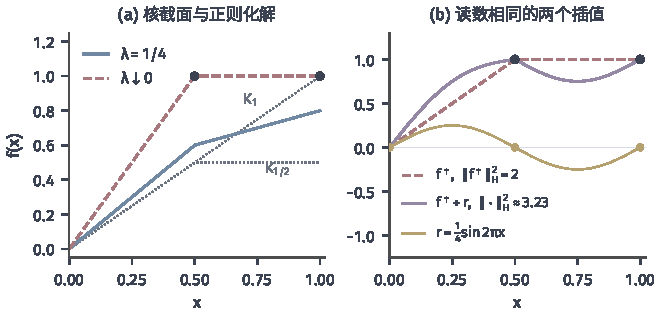
\includegraphics[width=112mm]{figures/03-optimization-evolution-and-signals/01-optimization/matplotlib/c8-min-kernel-fit/figure.pdf}
  \caption{最小值核$K(s,t)=\min(s,t)$空间中读$f(\tfrac12)=f(1)=1$（黑点）。(a)~灰色点线为核截面$K_{1/2}$与$K_1$；蓝线为$\lambda=\tfrac14$的正则化解$f_\lambda=\tfrac45K_{1/2}+\tfrac25K_1$，读数为$\tfrac35,\tfrac45$；红色虚线为$\lambda\downarrow0$的极限，即最小范数插值$f^\dagger=2K_{1/2}$。(b)~$f^\dagger$与另一个插值$f^\dagger+r$，$r=\tfrac14\sin2\pi x$在$0,\tfrac12,1$处为零（黄点）；两者读数相同，范数平方分别为$2$与$2+\pi^2/8\approx3.23$。}
  \label{fig:opt-fit-min-kernel}
\end{figure}

\subsection{一般损失下的拟合}
\label{sec:opt-fit-general-loss}

\paragraph{先选损失，再用表示定理}
读数含离群值时，可以把式~\eqref{eq:opt-fit-kernel-ridge}中的平方换成绝对值或Huber损失：
\[
  J(f)=\frac1n\sum_{i=1}^n\ell(L_if-y_i)+\lambda\|f\|_H^2 .
\]
损失的选择取决于对读数误差的判断，与表示定理无关；选定以后，表示定理照样适用，因为它对数据代价$\Phi$没有任何要求。于是问题化为系数形式$J(\bm a)=\frac1n\sum_i\ell((\bm G\bm a)_i-y_i)+\lambda\bm a^\top\bm G\bm a$：Huber损失光滑，可以用第~\ref{chap:opt-smooth}章的梯度或牛顿型方法；绝对值损失不可微，可以用第~\ref{chap:opt-nonsmooth}章的次梯度与邻近方法，或第~\ref{sec:opt-fit-irls}小节的IRLS。

\paragraph{存在与唯一}
设$\ell$凸且连续，$\lambda>0$。先看存在性：$J(f)\ge\lambda\|f\|_H^2$（损失非负时；一般地$\ell$有仿射下界也可类似处理），所以$J$在$M$上强制，即$\|f\|_H\to\infty$时$J(f)\to\infty$。$M$是有限维空间，$J$在$M$上连续，于是任一下水平集$\{f\in M:J(f)\le J(0)\}$是有界闭集，因而是紧集，$J$在其上达到最小值；由表示定理第1条，这也是$H$上的最小值。再看唯一性：$\lambda\|f\|_H^2$严格凸，加上凸的数据项，$J$在$H$上严格凸，至多有一个最小点。所以对凸连续损失，最优函数存在且唯一；系数则仍可能沿$\ker\bm G$不唯一。对非凸损失（例如Cauchy代价），表示定理的第2、3条仍说明最小点若存在可取在$M$中，但存在性与唯一性都需要另外检查，不能只凭有限表示得到同样的结论。

\paragraph{观测数很大时的计算方式}
上面的有限维问题有$n$个未知数，但Gram矩阵有$n^2$个元素。$n=10^5$时，双精度存储$\bm G$需要$8\times10^{10}$字节，约$80$\,GB，而Cholesky分解还需要约$n^3/3\approx3\times10^{14}$次运算。迭代方法只需要矩阵向量积$\bm G\bm a$：每个分量$(\bm G\bm a)_i=\sum_ja_jL_ih_j$可以在需要时重新计算核值，存储降到$O(n)$，每次乘积的计算量仍是$O(n^2)$次核求值。能否进一步避免显式矩阵，取决于观测与核的结构，例如规则网格上的平移不变核可以借助快速Fourier变换。用有限个特征近似核，或者让迭代提前停止，会带来不同性质的误差，第~\ref{sec:opt-fit-representation-computation}小节统一比较；核空间的构造与谱特征的依据见前文引用的卷二“再生核Hilbert空间”章。
